% SPDX-License-Identifier: CC-BY-4.0
\documentclass[12pt,letterpaper]{article}
\usepackage[T1]{fontenc}
\usepackage{amsmath,amssymb,amsthm}
\usepackage{newtxtext,newtxmath}
\usepackage[margin=1in]{geometry}
\usepackage{microtype,booktabs,tikz,array}
\usetikzlibrary{matrix,positioning,calc}
\usepackage[hidelinks]{hyperref}
\newtheorem{theorem}{Theorem}[section]
\newtheorem{proposition}[theorem]{Proposition}
\newtheorem{lemma}[theorem]{Lemma}
\theoremstyle{definition}\newtheorem{example}[theorem]{Example}
\numberwithin{equation}{section}
\newcommand{\F}{\mathbf F}
\DeclareMathOperator{\PSL}{PSL}
\DeclareMathOperator{\supp}{supp}
\tikzset{mymat/.style={matrix of nodes,nodes in empty cells,nodes={minimum width=.75cm,minimum height=.75cm,anchor=center},column sep=-\pgflinewidth,row sep=-\pgflinewidth,ampersand replacement=\&}}

\title{MINIMOGs and Mathematical Blackjack\\\large Draft 2: Corrected and expanded version}
\author{David Joyner\thanks{Original manuscript dated May 29, 2000. Corrected and expanded November 26, 2026.}\\\small\texttt{wdjoyner@gmail.com}}
\date{Original draft: 2000. Corrected and expanded draft: 2026}

\begin{document}
\maketitle

\begin{abstract}
This AI-aided paper used ChatGPT to referee, revise, and expand the original manuscript (see the acknowledgments). We describe the small Witt design using the projective line over $\F_{11}$, Curtis's kitten, and Conway's MINIMOG. The tetracode gives a compact membership test for hexads. We explain mathematical blackjack through a directed Johnson graph, prove an extremal independent-set result, and give an exact verification of the constructions and game strategy. We also compute the conditional probability of winning under the redealing rule.
\end{abstract}

\tableofcontents

\section{Introduction}
A collection of six-element subsets of a twelve-element set can have the remarkable property that every five-element subset belongs to exactly one member. This is the small Witt design. Its blocks, called hexads, admit several descriptions which appear at first to have little in common. The purpose of this paper is to explain their equivalence and their application to a card game.

For example, in the shuffle numbering, $\{1,2,3,4,5,6\}$ is a hexad. Its complement is also a hexad. In mathematical blackjack these two hands are losing positions for the player about to move, despite their very different totals. We explain this phenomenon using an orientation of a graph on six-element subsets.

The main results are the equivalence of the three explicit constructions (Sections~\ref{sec:projective}--\ref{sec:shuffle}), an equitable partition and sharp independence bound for the Johnson graph (Section~\ref{sec:graph}), and a kernel description of the game (Section~\ref{sec:game}). The finite computations used in the proofs are reproduced by the accompanying standard-library Python script \texttt{verify.py}.

\subsection{Literature review}
The historical constructions motivate both the geometric and coding-theoretic approaches. They also show why the small Witt design sits naturally at the meeting point of finite geometry, coding theory, and combinatorial game theory.

\subsubsection*{Work before 2000}
Curtis's construction of the MOG for the large Witt design \cite{Cu76} and his kitten for the small Witt design \cite{Cu84} provide explicit geometric descriptions of the Mathieu groups' designs. Conway's tetracode and MINIMOG \cite{Co84} encode the small design using a rectangular array. Conway and Sloane \cite[Chapter 11, p.~321]{CS99} describe these patterns in the context of codes and lattices. For example, a four-coordinate tetracode word specifies one cell in each MINIMOG column. The relationship between games and codes is developed in \cite{CS86}, while normal-play game terminology is treated in \cite{Co76}.

\subsubsection*{Work after 2000}
Kahane and Ryba's \emph{The Hexad Game} \cite{KR01} gives a non-enumerative proof of the hexad-game theorem and studies nim sums and Welter values. Irie \cite{Ir21} constructs games from Steiner systems and characterizes the shuffle design by minimizing the number of game positions among the 5040 labeled designs. This is a different, complementary perspective to our fixed Johnson graph orientation. The author's 2006 implementation, documented in the SageMath reference manual \cite{Jo06}, supplies the module \texttt{sage.games.hexad}, which implements hexad completion and blackjack moves. For instance, the method \texttt{find\_hexad} provides an alternative to searching the entire set of blocks. The present exposition uses a separate exhaustive Python verification so that no specialized mathematics software is required.

\subsection{Notation}
The following notation distinguishes the abstract design from its numerical labelings. For example, the symbol $\infty$ belongs to the projective labeling, not to a card hand.

\begin{center}
\begin{tabular}{ll}\toprule
Symbol & Meaning\\\midrule
$X$ & Twelve-point set, usually $\{0,\ldots,11\}$\\
$\mathcal H$ & Family of hexads\\
$\F_q$ & Finite field with $q$ elements\\
$T$ & Tetracode over $\F_3$\\
$J(n,k)$ & Johnson graph on $k$-subsets of an $n$-set\\
$w(A)$ & Sum of the card labels in $A$\\
$\mathcal P,\mathcal N$ & Losing and winning positions for the next player\\\bottomrule
\end{tabular}
\end{center}

\section{Background}\label{sec:background}
We collect the elementary notions used in the constructions and the later graph interpretation. The two subsections of this background are meant to orient a reader who knows some algebra and combinatorics but has not worked specifically with the Witt design.

\subsection{Designs and finite geometry}
A Steiner system $S(t,k,n)$ consists of an $n$-element set $X$ and a family $\mathcal H$ of $k$-element subsets such that every $t$-element subset belongs to exactly one block. For example, the seven lines of the projective plane over $\F_2$ form an $S(2,3,7)$. The small Witt design is an $S(5,6,12)$. Its uniqueness up to relabeling is a classical fact \cite{Cu84}. Its automorphism group is the Mathieu group $M_{12}$.

The Fano plane in Figure~\ref{fig:fano} is the standard example of an $S(2,3,7)$. Every two points determine a unique line, and each line has three points. This is a useful model to keep in mind because it shows, on a very small scale, the design principle that also governs the Witt design. The kitten pictures below play a somewhat analogous role for $S(5,6,12)$: they make a highly symmetric Steiner system visible inside familiar finite geometry.

\begin{figure}[ht]
\centering
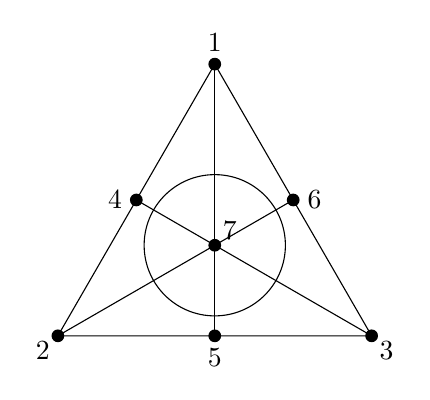
\begin{tikzpicture}[scale=1.15, every node/.style={circle,fill,inner sep=1.8pt}]
\coordinate (A) at (90:2);
\coordinate (B) at (210:2);
\coordinate (C) at (330:2);
\coordinate (AB) at ($(A)!0.5!(B)$);
\coordinate (BC) at ($(B)!0.5!(C)$);
\coordinate (CA) at ($(C)!0.5!(A)$);
\coordinate (O) at (0,0);
\draw (A)--(B)--(C)--cycle;
\draw (A)--(BC);
\draw (B)--(CA);
\draw (C)--(AB);
\draw (0,0) circle (0.78);
\foreach \P/\name/\pos in {A/1/above, B/2/below left, C/3/below right, AB/4/left, BC/5/below, CA/6/right, O/7/above right}{
  \fill (\P) circle (2pt);
  \node[draw=none,fill=none,inner sep=1pt,\pos=2pt] at (\P) {$\name$};}
\end{tikzpicture}
\caption{The Fano plane, the smallest projective plane, viewed as an $S(2,3,7)$.}
\label{fig:fano}
\end{figure}

The projective line $\mathbf P^1(\F_q)$ is the set of one-dimensional subspaces of $\F_q^2$. It may be written $\F_q\cup\{\infty\}$. For instance, the point $\infty$ is represented by $(1,0)$ and a finite point $x$ by $(x,1)$. The affine plane $\F_3^2$ has nine points. Its lines are solutions of $ar+bc=d$ with $(a,b)\ne(0,0)$. For example, $r+c=0$ contains $(0,0),(1,2),(2,1)$.

\subsection{Codes and graphs}
A linear $[n,k,d]$ code over $\F_q$ is a $k$-dimensional subspace of $\F_q^n$ with minimum nonzero Hamming weight $d$. The Hamming weight counts nonzero coordinates. For example, the span of $(1,1,1)$ over $\F_3$ is a $[3,1,3]$ code.

The tetracode used later in the MINIMOG has a convenient basis in standard form. One may take the generator matrix
\begin{equation}\label{eq:tetrastandard}
G=\begin{pmatrix}1&0&1&2\\0&1&1&1\end{pmatrix}.
\end{equation}
Thus a message vector $(u,v)\in\F_3^2$ produces the codeword
\[
(u,v)G=(u,v,u+v,2u+v).
\]
For example, $(2,1)G=(2,1,0,2)$. In the MINIMOG this codeword singles out the row pattern $(-,+,0,-)$, one chosen row in each of the four columns. Later, such patterns encode the allowed odd-man-out coordinates for a hexad.

A graph is a set of vertices with a specified adjacency relation. An independent set contains no adjacent pair. A partition is equitable if every vertex in a given class has the same number of neighbors in each class. For example, the two parts of the complete bipartite graph $K_{2,3}$ form an equitable partition with quotient matrix $\left(\begin{smallmatrix}0&3\\2&0\end{smallmatrix}\right)$. We shall see that the 132 hexads form an independent set in a Johnson graph, and that the design induces an equitable partition of that graph.

\section{The projective-line construction}\label{sec:projective}
We first construct the blocks as an orbit under fractional linear transformations. Set
\[
Q=\{0,1,3,4,5,9\}\subset\mathbf P^1(\F_{11}),
\qquad \alpha(x)=x+1,\quad\beta(x)=-1/x.
\]
Here $\alpha(\infty)=\infty$, $\beta(0)=\infty$, and $\beta(\infty)=0$. The set $Q$ consists of zero and the nonzero squares modulo 11. The two transformations generate $\PSL(2,11)$: their matrices give upper and lower elementary unipotent matrices by taking powers and conjugating. These generate $\mathrm{SL}(2,11)$ by elementary row reduction, and passing to projective transformations gives the assertion.

\begin{lemma}\label{lem:orbit}
The orbit of $Q$ under $\langle\alpha,\beta\rangle$ is an $S(5,6,12)$.
\end{lemma}

\begin{proof}[Proof by exact finite enumeration]
Start with $Q$ in a queue and apply both generators to each newly discovered subset until the queue is empty. The output is the entire orbit since the two permutations have finite order and their inverses are positive powers. The script \texttt{verify.py} implements this procedure and counts the five-subsets of every output block. It gives 132 distinct blocks and 792 distinct five-subsets, each with multiplicity one. Since $\binom{12}{5}=792$, the defining property follows. All computations use integers and finite sets.
\end{proof}

For example, applying $\alpha$ gives $\{1,2,4,5,6,10\}$.

\begin{proposition}\label{prop:parameters}
The number of hexads containing any fixed $j$-subset is
\begin{equation}\label{eq:lambda}
\lambda_j=\frac{\binom{12-j}{5-j}}{\binom{6-j}{5-j}},\qquad 0\le j\le5.
\end{equation}
Every hexad has a hexad as its complement.
\end{proposition}

\begin{proof}
Count five-subsets containing the prescribed $j$-subset, first directly and then inside their unique hexads. This gives \eqref{eq:lambda}, with values $132,66,30,12,4,1$. Fix a hexad $B$ and let $n_i$ count other hexads meeting it in $i$ points. Then $n_5=0$ and
\[
\sum_{i=j}^4\binom{i}{j}n_i=\binom{6}{j}(\lambda_j-1)\qquad(0\le j\le4).
\]
Solving successively from $j=4$ down to zero gives $(n_0,n_1,n_2,n_3,n_4)=(1,0,45,40,45)$. The unique disjoint hexad is the complement of $B$.
\end{proof}

\section{Curtis's kitten}\label{sec:kitten}
The kitten replaces the twelve-point orbit by three pictures on the same nine ordinary points. The distinguished points are $D=\{\infty,0,1\}$. Figure~\ref{fig:kitten-threeviews} redraws the three projective kitten pictures in TikZ. These are the three affine views used to generate the four hexad types.

\begin{figure}[ht]
\centering
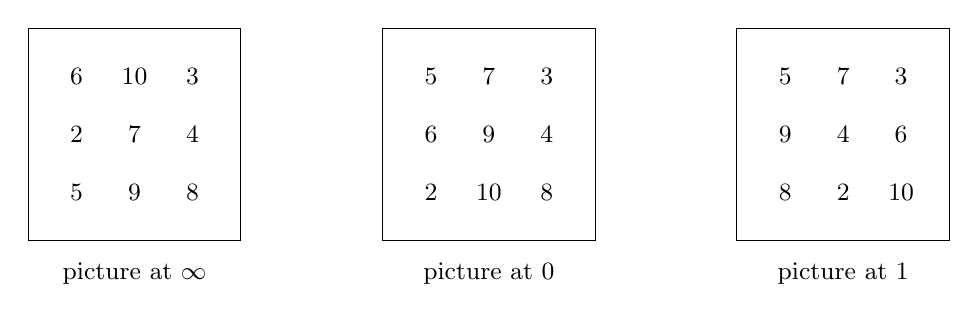
\begin{tikzpicture}[every node/.style={font=\small},
  box/.style={draw,minimum width=2.7cm,minimum height=2.7cm,inner sep=0pt}]
\node[box] (A) at (0,0) {};
\matrix[mymat] at (A.center) {
6 \& 10 \& 3\\
2 \& 7 \& 4\\
5 \& 9 \& 8\\
};
\node[below=.15cm of A] {picture at $\infty$};

\node[box] (B) at (4.5,0) {};
\matrix[mymat] at (B.center) {
5 \& 7 \& 3\\
6 \& 9 \& 4\\
2 \& 10 \& 8\\
};
\node[below=.15cm of B] {picture at $0$};

\node[box] (C) at (9,0) {};
\matrix[mymat] at (C.center) {
5 \& 7 \& 3\\
9 \& 4 \& 6\\
8 \& 2 \& 10\\
};
\node[below=.15cm of C] {picture at $1$};
\end{tikzpicture}
\caption{Curtis's kitten in its three affine views.}
\label{fig:kitten-threeviews}
\end{figure}

Figure~\ref{fig:kitten-schematic} gives a second diagram, adapted from the kitten figure in the earlier exposition. It emphasizes the three distinguished points and the triangular way in which one passes among the three affine pictures.

\begin{figure}[ht]
\centering
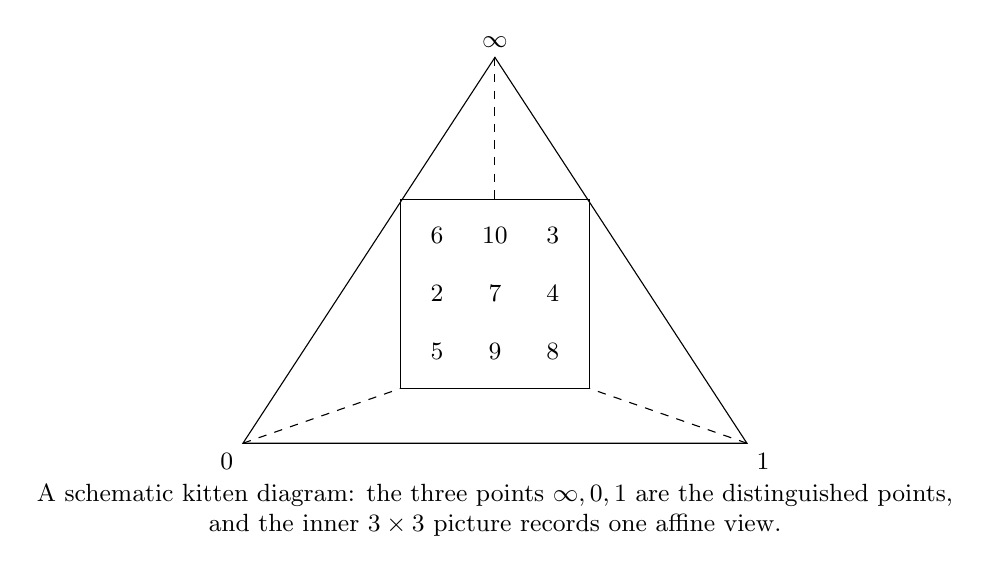
\begin{tikzpicture}[scale=1, every node/.style={font=\small}]
\coordinate (Top) at (0,3.2);
\coordinate (L) at (-3.2,-1.7);
\coordinate (R) at (3.2,-1.7);
\draw (Top)--(L)--(R)--cycle;
\node[above] at (Top) {$\infty$};
\node[below left] at (L) {$0$};
\node[below right] at (R) {$1$};

\node[draw,minimum width=2.4cm,minimum height=2.4cm,inner sep=0pt] (M) at (0,.2) {};
\matrix[mymat] at (M.center) {
6 \& 10 \& 3\\
2 \& 7 \& 4\\
5 \& 9 \& 8\\
};
\draw[dashed] (Top) -- (M.north);
\draw[dashed] (L) -- (M.south west);
\draw[dashed] (R) -- (M.south east);
\node[align=center] at (0,-2.55) {A schematic kitten diagram: the three points $\infty,0,1$ are the distinguished points,\\ and the inner $3\times 3$ picture records one affine view.};
\end{tikzpicture}
\caption{A schematic TikZ redrawing of Curtis's kitten.}
\label{fig:kitten-schematic}
\end{figure}

Each picture is an affine plane with row and column coordinates in $\F_3$. There are four directions, each with three parallel lines. With respect to the dot product, the horizontal and vertical directions are perpendicular, as are the two diagonal directions. A cross is the union of two perpendicular lines. Each direction pair gives nine crosses, since each line can be chosen in three ways. The complement of a cross is called a square. Figure~\ref{fig:cross} shows the two types of crosses.

\begin{figure}[ht]
\centering
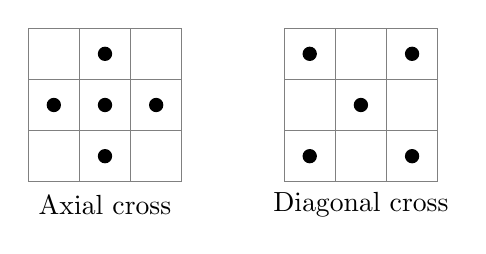
\begin{tikzpicture}[scale=.65]
\foreach \s in {0,5}{\begin{scope}[xshift=\s cm]\draw[step=1,gray] (0,0) grid (3,3);\foreach \x in {0,1,2}{\foreach \y in {0,1,2}{\ifnum\s=0\ifnum\x=1\fill (\x+.5,\y+.5) circle (.14);\else\ifnum\y=1\fill (\x+.5,\y+.5) circle (.14);\fi\fi\else\ifnum\x=\y\fill (\x+.5,\y+.5) circle (.14);\else\pgfmathtruncatemacro{\z}{\x+\y}\ifnum\z=2\fill (\x+.5,\y+.5) circle (.14);\fi\fi\fi}}\end{scope}}
\node at (1.5,-.45){Axial cross};\node at (6.5,-.45){Diagonal cross};
\end{tikzpicture}
\caption{Two types of crosses. Their translates give all eighteen crosses in a picture.}
\label{fig:cross}
\end{figure}

Curtis's four types of hexads \cite{Cu84} are:
\begin{enumerate}
\item All three distinguished points together with a line in a picture.
\item Two distinct parallel lines in a picture.
\item A distinguished point together with a cross in its picture.
\item Two distinguished points together with a square in the picture at the omitted distinguished point.
\end{enumerate}
The first two collections are the same in all three pictures: their lines, as sets, coincide. Each therefore has twelve members. The third and fourth types each have $3\cdot18=54$ members. They are disjoint by their numbers of distinguished points. For example, the first row in the picture at $\infty$ gives $\{\infty,0,1,6,10,3\}$. Equality of the resulting 132 blocks with the orbit is verified in Section~\ref{sec:shuffle}.

\section{The MINIMOG and tetracode}\label{sec:minimog}
Conway's MINIMOG encodes hexads in a $3\times4$ array. Its row labels are $0,1,2$, also written $0,+,-$. We first review the tetracode in a way adapted to the later membership test.

\subsection{The tetracode}
Define
\begin{equation}\label{eq:tetracode}
T=\{(b,a,a+b,a+2b):a,b\in\F_3\}.
\end{equation}
Using the ordered basis from \eqref{eq:tetrastandard}, the same code is generated by
\[
\begin{pmatrix}1&0&1&2\\0&1&1&1\end{pmatrix}.
\]
Any two columns are linearly independent, so any two coordinate values determine a word. Every nonzero word has exactly one zero coordinate: if $b=0$ the first coordinate is zero, and otherwise exactly one of $a,a+b,a+2b$ vanishes. Hence $T$ is a $[4,2,3]$ code with weight enumerator $1+8z^3$. The generator rows have zero dot products with each other and themselves, so the dimension-two code is self-dual.

For example, the message $(2,1)$ produces the word $(2,1,0,2)$. If the four row labels are read as $(0,+,-)$ for $(0,1,2)$, then this word means ``choose row $-$ in the first column, row $+$ in the second, row $0$ in the third, and row $-$ in the fourth.'' This is precisely the kind of row pattern that appears in the MINIMOG test.

\subsection{The membership test}
The shuffle MINIMOG is
\begin{equation}\label{eq:shuffle}
\begin{array}{c|rrrr}0&6&3&0&9\\+&5&2&7&10\\-&4&1&8&11\end{array}.
\end{equation}
For a six-subset, the odd man out is the occupied row if a column has one selected cell, and the unoccupied row if it has two. A full or empty column contributes a wildcard (Figure~\ref{fig:odd}). The subset passes the test if the column counts are not a permutation of $(0,1,2,3)$ and the specified coordinates extend to a word in $T$.

\begin{figure}[ht]
\centering
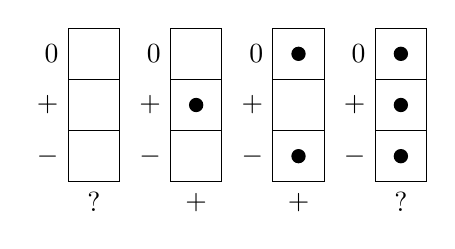
\begin{tikzpicture}[scale=.65]
\foreach \c/\s/\lab in {0/0/{?},2/1/{+},4/2/{+},6/3/{?}}{\begin{scope}[xshift=\c cm]\draw[step=1] (0,0) grid (1,3);\foreach \r in {0,1,2}{\node[left] at (0,2.5-\r){\ifcase\r $0$\or $+$\or $-$\fi};\ifnum\s=1\ifnum\r=1\fill (.5,2.5-\r) circle (.14);\fi\fi\ifnum\s=2\ifnum\r=1\else\fill (.5,2.5-\r) circle (.14);\fi\fi\ifnum\s=3\fill (.5,2.5-\r) circle (.14);\fi}\node at (.5,-.4){$\lab$};\end{scope}}
\end{tikzpicture}
\caption{Odd-man-out coordinates for the four column occupancies.}
\label{fig:odd}
\end{figure}

\begin{lemma}\label{lem:minimog}
The membership test selects precisely the 132 shuffle hexads, after the relabeling of Section~\ref{sec:shuffle}.
\end{lemma}

\begin{proof}
The exact enumeration in \texttt{verify.py} loops over all 924 six-subsets, rejects the prohibited occupancy pattern, and tests the remaining specified rows against the nine words in \eqref{eq:tetracode}. It compares the resulting family with the relabeled orbit from Lemma~\ref{lem:orbit} and obtains equality. Section~\ref{sec:shuffle} specifies the bijection used in this comparison.
\end{proof}

For example, the first two full columns give $\{1,2,3,4,5,6\}$ with four wildcards, so the test accepts it. In contrast, a full column, a double column, a single column and an empty column are rejected regardless of their row labels.

\subsection{Signed patterns}
The original signed construction \cite{CS99} uses a column vector $C_i$ with ones in column $i$ and a tetrad vector $U_t$ with ones in the four cells specified by $t\in T$. Regard the arrays as vectors over $\F_3$. Take the supports of
\[
C_i-C_j,\quad C_i+U_t,\quad U_t-U_u,\quad C_i+C_j-U_t,
\]
where $i\ne j$ and $t\ne u$ in the relevant expressions. These supports are precisely the 132 hexads, as checked by the same script. For instance, $C_1-C_2$ represents the signed entries $4,5,6,-1,-2,-3$. For $t=(0,1,1,1)$ the vector $C_2+U_t$ has support $\{1,2,3,6,7,10\}$, with coefficient $-1$ at 2 and coefficient $+1$ elsewhere. Signs are coefficients of cells, so the sign at card zero is meaningful even though its integer label is zero.

\section{The shuffle kitten}\label{sec:shuffle}
The projective MINIMOG is
\[
\begin{array}{rrrr}0&3&\infty&2\\5&9&8&10\\4&1&6&7\end{array}.
\]
Matching cells with \eqref{eq:shuffle} defines a bijection from the projective labels to shuffle labels. In particular, $0\mapsto6$, $1\mapsto1$, and $\infty\mapsto0$. The corresponding pictures, with the distinguished point indicated below each, are
\[
\begin{array}{c@{\qquad}c@{\qquad}c}
\begin{array}{ccc}5&11&3\\8&2&4\\9&10&7\end{array}&
\begin{array}{ccc}5&11&3\\2&4&8\\7&9&10\end{array}&
\begin{array}{ccc}8&10&3\\9&11&4\\5&2&7\end{array}\\6&1&0
\end{array}
\]
The script constructs the four kitten families by enumerating the twelve affine lines in each picture and the eighteen perpendicular pairs. It checks the counts $12,12,54,54$ and equality of their union with the relabeled projective orbit and with the MINIMOG family. This proves the equivalence of the explicit descriptions by exact finite enumeration.

For example, $\{2,4,5,11\}$ is the complement of a cross in the picture at 1, giving the hexad $\{0,2,4,5,6,11\}$. The cross $\{2,3,4,5,7\}$ in the picture at 0 gives the hexad $\{0,2,3,4,5,7\}$.

\section{The Johnson graph and the Witt design}\label{sec:graph}
The geometry of the design has a simple graph-theoretic expression. The Johnson graph $J(n,k)$ has the $k$-subsets of an $n$-set as vertices, with adjacency when two subsets differ in one element. For example, $\{1,2\}$ and $\{1,3\}$ are adjacent in $J(4,2)$. Here $J(12,6)$ has 924 vertices of degree 36.

\begin{theorem}\label{thm:equitable}
The hexads form a maximum independent set of $J(12,6)$. The partition into hexads and nonhexads is equitable with quotient matrix
\begin{equation}\label{eq:quotient}
B=\begin{pmatrix}0&36\\6&30\end{pmatrix}.
\end{equation}
\end{theorem}

\begin{proof}
Two distinct hexads cannot contain the same five-subset, so no two are adjacent. For a nonhexad $A$, each of its six five-subsets has a unique hexad completion. These completions are distinct, since a block containing two of the five-subsets would contain their union $A$ and hence equal $A$. Each completion is adjacent to $A$, and all hexad neighbors arise this way. The quotient matrix follows. Figure~\ref{fig:quotient} illustrates the partition. Any independent set of six-subsets uses disjoint collections of five-subsets. Its size is therefore at most $\binom{12}{5}/6=132$, attained by the design.
\end{proof}

\begin{figure}[ht]
\centering
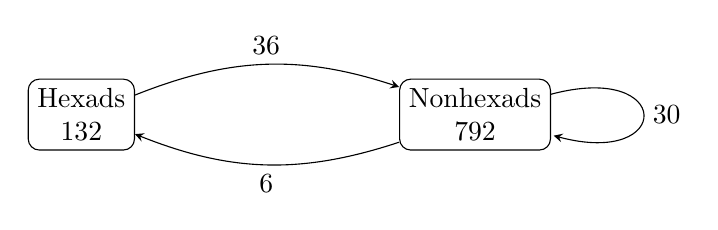
\begin{tikzpicture}[>=stealth]
\node[draw,rounded corners,align=center] (h) at (0,0){Hexads\\132};
\node[draw,rounded corners,align=center] (n) at (5,0){Nonhexads\\792};
\draw[->] (h) to[bend left=20] node[above]{36} (n);
\draw[->] (n) to[bend left=20] node[below]{6} (h);
\draw[->] (n) edge[loop right] node[right]{30} (n);
\end{tikzpicture}
\caption{Equitable quotient. Labels count neighbors per vertex.}
\label{fig:quotient}
\end{figure}

There is also a spectral explanation. Let $W$ be the incidence matrix with rows indexed by five-subsets and columns by six-subsets, with entries 1 for containment and 0 otherwise. If $A_J$ is the adjacency matrix, then $W^\mathsf{T}W=6I+A_J$. Thus every eigenvalue of $A_J$ is at least $-6$. The quotient matrix has eigenvalues 36 and $-6$, which lift to the graph by taking vectors constant on each class. Hence $-6$ is the smallest eigenvalue. For an independent set of size $s$, subtract $(s/924)\mathbf 1$ from its indicator vector and apply the lower eigenvalue bound to its quadratic form. This gives
\[
-36s^2/924\ge -6(s-s^2/924),
\]
so $s\le132$. The design attains the spectral bound as well as the elementary counting bound.

\section{Mathematical blackjack}\label{sec:game}
The shuffle numbering makes the hexads the losing positions of a particular impartial game. We give precise rules and an exact proof of the strategy attributed to Conway and Ryba \cite{CS86,KR01}.

\subsection{Rules and directed graph}
There are twelve cards labeled $0,\ldots,11$. A hand is a six-subset $A$, visible to both players, with the remaining cards available in a shared pile. A legal position satisfies $w(A)=\sum_{a\in A}a\ge21$. Players alternate replacing $a\in A$ by $b\notin A$ with $b<a$ and with the new total at least 21. A player with no legal move loses. Equivalently, a move below 21 can be treated as an immediate loss for its maker. For random play of the initial deal, shuffle and redeal whenever the initial total is at most 21.

Orient each edge of $J(12,6)$ from the larger total to the smaller total and delete all vertices of total less than 21. This gives a finite acyclic graph. A kernel is an independent set such that every outside vertex has an outgoing edge to the set. In an acyclic game graph, the kernel is exactly the set of $\mathcal P$-positions, since a player wins if and only if a move to a losing position exists.

\begin{theorem}\label{thm:game}
The shuffle hexads are precisely the kernel of the blackjack graph, and hence precisely the $\mathcal P$-positions.
\end{theorem}

\begin{proof}[Proof by exact finite enumeration]
By Theorem~\ref{thm:equitable}, the hexads are independent. The script enumerates all 905 legal positions in increasing total and applies the forced recursion just described. Since every legal move decreases the total, every possible successor has already been processed. The resulting kernel consists of exactly the 132 hexads from Lemma~\ref{lem:minimog}. This proves absorption and independence for the stated labeling. Independence alone would not imply absorption for an arbitrary labeling.
\end{proof}

\subsection{A worked game}
The original example illustrates the strategy. The initial hand $\{0,2,4,6,7,11\}$ has total 30 and odd-man-out coordinates $(1,1,2,2)$, which do not form a tetracode word. The following moves are possible.

\begin{center}
\begin{tabular}{clrl}\toprule
Move&Hand&Total&Class\\\midrule
Initial&$0,2,4,6,7,11$&30&$\mathcal N$\\
$7\to5$&$0,2,4,5,6,11$&28&$\mathcal P$\\
$11\to7$&$0,2,4,5,6,7$&24&$\mathcal N$\\
$6\to3$&$0,2,3,4,5,7$&21&$\mathcal P$\\\bottomrule
\end{tabular}
\end{center}

The second hand is a square together with two distinguished points. Its specified odd-man-out coordinates are $(?,1,0,2)$, which extend to $(2,1,0,2)$. The third hand has the prohibited occupancy pattern. The fourth hand is a cross together with one distinguished point. Its total is 21 and it has no legal successor. The first player wins. A separate way to find a winning move is to use the author's SageMath module \cite{Jo06}. For example, the documented command
\begin{verbatim}
from sage.games.hexad import Minimog
M = Minimog(type="shuffle")
M.blackjack_move([0, 2, 4, 6, 7, 11])
\end{verbatim}
returns the alternative winning exchange $4\to3$, reducing the total to 29. Our accompanying Python script does not require SageMath.

\subsection{Probability and the weight enumerator}
The sum of all twelve labels is 66. Proposition~\ref{prop:parameters} implies that the polynomial $F(t)=\sum_{H\in\mathcal H}t^{w(H)}$ satisfies
\begin{equation}\label{eq:reciprocity}
F(t)=t^{66}F(t^{-1}).
\end{equation}
Exact enumeration gives the coefficients for weights up to 33 below. The remaining coefficients follow by symmetry, and the coefficients outside $[21,45]$ vanish.

\begin{center}\small
\begin{tabular}{c|rrrrrrrrrrrrr}
Weight&21&22&23&24&25&26&27&28&29&30&31&32&33\\\hline
Count&11&0&0&2&2&4&4&6&6&8&8&10&10
\end{tabular}
\end{center}

For example, there are eleven terminal hexads of total 21 and eleven complementary hexads of total 45.

\begin{proposition}\label{prop:probability}
With a uniform initial six-subset and redealing until its total exceeds 21, the probability that the first player has a winning strategy is $773/894$.
\end{proposition}

\begin{proof}
Among the 924 hands, 19 have total below 21 and 11 have total exactly 21. These counts follow by enumerating the six-subsets, as in the script. All eleven hands of total 21 are hexads by Theorem~\ref{thm:game}. The uniform conditional sample has $924-30=894$ hands, including $132-11=121$ losing hands. The probability is $(894-121)/894=773/894$.
\end{proof}

If the deal is instead conditioned on total at least 21, the probability is $773/905$. Without conditioning, the probability of receiving a nonhexad is $6/7$, but nineteen of those nonhexads are below the legal threshold.

\section{Summary and future directions}
The projective orbit, kitten and MINIMOG describe the same small Witt design. The design is a maximum independent set of the Johnson graph and gives an equitable partition. The shuffle numbering also makes it the kernel of a natural acyclic orientation. For example, the six distinct hexad completions of a nonhexad in the undirected graph explain why many candidate moves are available, while the game theorem guarantees at least one decreasing completion for a legal nonhexad.

The following are questions for further investigation rather than claims of novelty. Can the coefficients of $F(t)$ be derived without enumeration from the tetracode? Which permutations of the labels preserve the kernel property? Can a similar orientation produce useful games from other Steiner systems? For instance, the general $S(k-1,k,n)$ construction yields an independent set in $J(n,k)$ and $k$ block neighbors of every nonblock, but directed absorption requires further conditions.

\section{Glossary}
The terms below summarize the concepts used above. Examples refer to the small design whenever possible.
\begin{description}
\item[Affine plane.] A geometry of points and lines with unique parallels through a point outside a line. Over $\F_3$ it has nine points and twelve lines. The kitten pictures are affine planes in this sense. Their row, column, and diagonal directions organize the line, cross, and square constructions.

\item[Cross.] A union of two perpendicular lines in a kitten picture. It contains five points because the lines meet in one point. In the kitten construction, adjoining the corresponding distinguished point to a cross produces a hexad.

\item[Equitable partition.] A vertex partition with constant interclass neighbor counts. Equation~\eqref{eq:quotient} is an example. This means that every hexad has the same number of nonhexad neighbors, and every nonhexad has the same number of hexad neighbors.

\item[Hexad.] A six-point block of the small Witt design. Five points determine its unique completion. In the shuffle labeling the 132 hexads are exactly the losing hands of mathematical blackjack.

\item[Impartial game.] A game in which the available moves depend on the position, not on the identity of the player. Mathematical blackjack has this property because each player faces exactly the same move rule. The theory of $\mathcal P$- and $\mathcal N$-positions applies directly to such games.

\item[Independent set.] A set containing no adjacent vertices. The hexads form such a set in the Johnson graph. This is another way to say that two distinct hexads never share five points.

\item[Johnson graph.] The graph of fixed-size subsets with adjacency given by one exchange. It describes possible card exchanges before orientation and threshold restrictions. In this paper the relevant graph is $J(12,6)$ on all six-subsets of a twelve-element set.

\item[Kernel.] An independent and outward-absorbing set in a directed graph. In the blackjack graph it consists of the losing positions. Every vertex outside the kernel has an outgoing edge to it.

\item[Kitten.] Curtis's three affine pictures with three distinguished points. Lines, crosses, and squares generate its four block types. The kitten gives a very concrete finite-geometric model for the small Witt design.

\item[Mathematical blackjack.] The impartial game played on six cards chosen from $\{0,1,\dots,11\}$. A legal move replaces one chosen card by a smaller unchosen card while keeping the total at least 21. If no legal move is available, the player to move loses; equivalently, positions of total 21 are terminal.

\item[Mathieu group.] One of the sporadic simple Mathieu groups. The group $M_{12}$ acts as the full automorphism group of the small Witt design. Its symmetry explains why the design admits several elegant coordinate models.

\item[MINIMOG.] Conway's three-by-four array for hexad recognition. It uses a tetracode test on column occupancies. The name reflects its role as a miniature analogue of the Miracle Octad Generator.

\item[MOG.] Curtis's Miracle Octad Generator for the large Witt design. Its four-by-six array is an analogue of the MINIMOG. Although this paper concerns the smaller design, the terminology and point of view come directly from the MOG.

\item[Odd man out.] The single occupied or unoccupied row in a column with one or two selected cells. Full and empty columns impose no constraint. The four resulting row labels are the input for the tetracode membership test.

\item[Projective line.] The one-dimensional subspaces of a two-dimensional vector space. Over $\F_{11}$ there are twelve such subspaces. The projective-line orbit of the quadratic residues is the first construction of the small Witt design used in this paper.

\item[Quadratic residue.] A nonzero square in a finite field. The residues modulo 11 are $1,3,4,5,9$. Together with $0$, they form the initial hexad $Q$ whose orbit generates the design.

\item[Shuffle labeling.] The numbering of the MINIMOG adapted to blackjack. Unlike an arbitrary relabeling, it gives the directed absorption property. This special labeling is what makes the hexads coincide with the losing game positions.

\item[Square.] The four-point complement of a cross in a kitten picture. Adjoining the other two distinguished points gives a hexad. Squares are therefore the natural four-point shapes dual to crosses in the affine pictures.

\item[Steiner system.] A family of fixed-size blocks in which each subset of a prescribed smaller size lies in exactly one block. Here the parameters are $(5,6,12)$. The small Witt design is one of the classical exceptional Steiner systems.

\item[Tetracode.] The ternary self-dual $[4,2,3]$ linear code of Equation~\eqref{eq:tetracode}. Any two coordinates determine a word. In the MINIMOG it records one distinguished row choice in each of four columns.

\item[Witt design.] One of the exceptional Steiner systems associated with Mathieu groups. The small design has 132 blocks. It is unique up to relabeling and has unusually rich symmetry.

\item[$\mathcal P$- and $\mathcal N$-positions.] Positions losing or winning, respectively, for the next player under optimal normal play. Terminal positions belong to $\mathcal P$. In mathematical blackjack, the shuffle hexads are exactly the $\mathcal P$-positions.
\end{description}

\section*{Acknowledgments}
The author thanks Alex Ryba and Andy Buchanan for helpful comments on the original manuscript. ChatGPT refereed the manuscript, drafted the expanded exposition, derived the graph-theoretic arguments, and implemented and ran the finite verification. AI review is not an independent certification of the results. Further details on AI usage and source verification appear in the separate revision log.

\begin{thebibliography}{99}
\bibitem[Cu76]{Cu76} R. T. Curtis, A new combinatorial approach to $M_{24}$, Math. Proc. Cambridge Philos. Soc. \textbf{79} (1976), 25--42.
\bibitem[Cu84]{Cu84} R. T. Curtis, The Steiner system $S(5,6,12)$, the Mathieu group $M_{12}$, and the kitten, in \emph{Computational Group Theory}, M. Atkinson (ed.), Academic Press, 1984, pp.~353--358.
\bibitem[Co84]{Co84} J. H. Conway, Hexacode and tetracode---MOG and MINIMOG, in \emph{Computational Group Theory}, M. Atkinson (ed.), Academic Press, 1984, pp.~359--365.
\bibitem[Co76]{Co76} J. H. Conway, \emph{On Numbers and Games}, Academic Press, 1976.
\bibitem[CS86]{CS86} J. H. Conway and N. J. A. Sloane, Lexicographic codes: error-correcting codes from game theory, IEEE Trans. Inform. Theory \textbf{32} (1986), 337--348.
\bibitem[CS99]{CS99} J. H. Conway and N. J. A. Sloane, \emph{Sphere Packings, Lattices and Groups}, 3rd ed., Springer, 1999.
\bibitem[KR01]{KR01} J. Kahane and A. J. Ryba, The hexad game, Electron. J. Combin. \textbf{8} (2001), no. 2, Research Paper 11.
\bibitem[Ir21]{Ir21} Y. Irie, Combinatorial game distributions of Steiner systems, Electron. J. Combin. \textbf{28} (2021), no. 4, Paper 4.54.
\bibitem[Jo06]{Jo06} D. Joyner, SageMath, Hexads in $S(5,6,12)$, reference manual, \url{https://doc.sagemath.org/html/en/reference/games/sage/games/hexad.html}.
\end{thebibliography}

\end{document}
